\documentclass[border=2mm]{standalone}
\usepackage{tikz}
\usetikzlibrary{fit,positioning,arrows,automata}

\begin{document}

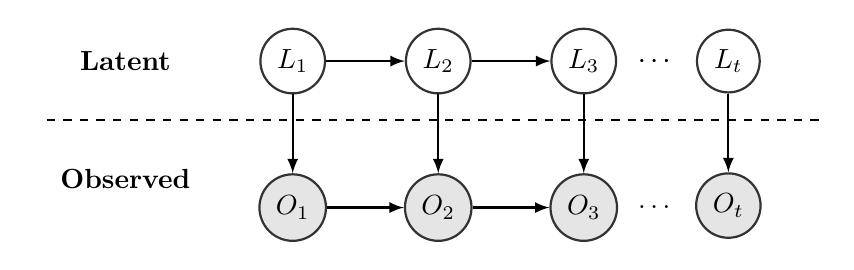
\begin{tikzpicture}
\tikzstyle{main}=[circle, minimum size = 5mm, thick, draw =black!80, node distance = 10mm]
\tikzstyle{connect}=[-latex, thick]
\tikzstyle{box}=[rectangle, draw=black!100]
  \node[box,draw=white!100] (Latent) {\textbf{Latent}};
  \node[main] (L1) [right=of Latent] {$L_1$};
  \node[main] (L2) [right=of L1] {$L_2$};
  \node[main] (L3) [right=of L2] {$L_3$};
  \node[main] (Lt) [right=of L3] {$L_t$};
  \node[box,draw=white!100] (Observed) [below=of Latent] {\textbf{Observed}};
    \node[main,fill=black!10] (O1) [right=of Observed,below=of L1] {$O_1$};
  \node[main,fill=black!10] (O2) [right=of O1,below=of L2] {$O_2$};
  \node[main,fill=black!10] (O3) [right=of O2,below=of L3] {$O_3$};
  \node[main,fill=black!10] (Ot) [right=of O3,below=of Lt] {$O_t$};
  \path (L3) -- node[auto=false]{\ldots} (Lt);
  \path (L1) edge [connect] (L2)
        (L2) edge [connect] (L3)
        (L3) -- node[auto=false]{\ldots} (Lt);
  \path (O1) edge [connect] (O2)
        (O2) edge [connect] (O3)
        (O3) -- node[auto=false]{\ldots} (Ot);
  \path (L1) edge [connect] (O1);
  \path (L2) edge [connect] (O2);
  \path (L3) edge [connect] (O3);
  \path (Lt) edge [connect] (Ot);
  \draw[dashed]  [below=of L1,above=of O1];

\path (Latent) -- (Observed) coordinate[midway](l44);
\node (l43) [left=of l44] {};
\path (Lt) -- (Ot) coordinate[midway](l444);
\node (l433) [right=of l444] {};
\draw[dashed,thick] (l43) to ++(0:10);

\end{tikzpicture}

\end{document}